\documentclass[cs4size,a4paper]{ctexart}   
%===数学符号公式===
\usepackage{amsmath}    					% AMS LaTeX宏包
\usepackage[style=1]{mdframed}
\usepackage{amsthm}
\usepackage{amssymb}
\usepackage{bm}                      	% 数学公式中的黑斜体
\usepackage{bbm}
\usepackage{amsfonts}
\usepackage{mathrsfs}                	% 英文花体字 体
\usepackage{bbding,manfnt}    			% 一些图标,如 \dbend
\usepackage{lettrine}                	% 首字下沉,命令\lettrine
\def\attention{\lettrine[lines=2,lraise=0,nindent=0em]{\large\textdbend\hspace{1mm}}{}}
\usepackage{longtable}
\usepackage{enumerate}
\usepackage[toc,page]{appendix}
\usepackage{geometry}         			% 页边距调整
\geometry{top=3.0cm,bottom=2.7cm,left=2.5cm,right=2.5cm}
\usepackage[colorinlistoftodos,prependcaption,textsize=small]{todonotes}
%===公式按章编号===
\numberwithin{equation}{section}
\numberwithin{table}{section}
\numberwithin{figure}{section}
%===基本格式预置===
\usepackage{fancyhdr}
\pagestyle{fancy}
\fancyhf{}  
\fancyhead[C]{\zihao{5}  \kaishu Linear Algebra Done Wrong}
\fancyfoot[C]{~\zihao{5} \thepage~}
\renewcommand{\headrulewidth}{0.75pt} 
\CTEXsetup[format={\centering\bfseries\zihao{-2}},name={第, 章}]{section}
\CTEXsetup[nameformat={\bfseries\zihao{3}}]{subsection}
\CTEXsetup[nameformat={\bfseries\zihao{4}}]{subsubsection}
%===图形支持宏包===
\usepackage{graphicx}        			% 嵌入png图像
\usepackage{subfigure}
\usepackage{float}
\graphicspath{{figure/}}
\usepackage{color,xcolor}     			% 支持彩色文本、底色、文本框等
\usepackage[colorlinks,linkcolor=blue,anchorcolor=blue,citecolor=blue]{hyperref}
%\usepackage{caption}
\usepackage[ruled,linesnumbered]{algorithm2e}
%\captionsetup{figurewithin=section}
%===源码和流程图===
\usepackage{listings,fontspec}         	% 粘贴源代码
\newfontfamily\consolas{Consolas}
\definecolor{mygreen}{rgb}{0,0.6,0}
\definecolor{mygray}{rgb}{0.5,0.5,0.5}
\definecolor{mymauve}{rgb}{0.58,0,0.82}
%===颜色===
\usepackage{color,xcolor}
\definecolor{dkgreen}{rgb}{0,0.6,0}
\definecolor{gray}{rgb}{0.5,0.5,0.5}
\definecolor{mauve}{rgb}{0.58,0,0.82}
\usepackage{xcolor}
\lstset{ %
%numberstyle=\tiny\monaco,
%numberstyle=\color[RGB]{0,192,192},
%backgroundcolor=\color{white},   		% choose the background color
backgroundcolor=\color[RGB]{245,245,244},
%backgroundcolor=\color[rgb]{1,1,0.76},
basicstyle=\footnotesize\consolas,       % size of fonts used for the code
identifierstyle=\footnotesize\consolas, 
columns=fullflexible,
breaklines=true,                 		% automatic line breaking only at whitespace
captionpos=b,                    		% sets the caption-position to bottom
tabsize=2,
commentstyle=\color{mygreen}\consolas,   % comment style
%commentstyle=\it\color[RGB]{0,96,96},
escapeinside={\%*}{*)},          		% if you want to add LaTeX within your code
keywordstyle=\color{blue}\consolas,      % keyword style
stringstyle=\color{mymauve}\consolas,    % string literal style
%stringstyle=\rmfamily\slshape\color[RGB]{128,0,0},
frame=single,
rulesepcolor=\color{red!20!green!20!blue!20},
%identifierstyle=\color{red},
language=c++,
framexleftmargin=1.9mm,
xleftmargin=0.4em,
frame=none,
showstringspaces=false,
numbers=none,
}

%--------------------
\hypersetup{hidelinks}
\usepackage{booktabs}  
\usepackage{shorttoc}
\usepackage{tabu,tikz}
\usepackage{float}
\usepackage{multirow}

\tabcolsep=1ex
\tabulinesep=\tabcolsep
\newlength\tikzboxwidth
\newlength\tikzboxheight
\newcommand\tikzbox[1]{%
        \settowidth\tikzboxwidth{#1}%
        \settoheight\tikzboxheight{#1}%
        \begin{tikzpicture}
        \path[use as bounding box]
                (-0.5\tikzboxwidth,-0.5\tikzboxheight)rectangle
                (0.5\tikzboxwidth,0.5\tikzboxheight);
        \node[inner sep=\tabcolsep+0.5\arrayrulewidth,line width=0.5mm,draw=black]
                at(0,0){#1};
        \end{tikzpicture}%
        }
\makeatletter
\def\hlinew#1{%
  \noalign{\ifnum0=`}\fi\hrule \@height #1 \futurelet
   \reserved@a\@xhline}
   
\usepackage{CJK}
\usepackage{ifthen}
\newcommand{\HRule}{\rule{\linewidth}{0.5mm}}
\newcommand{\tabincell}[2]{\begin{tabular}{@{}#1@{}}#2\end{tabular}}%
%===使得公式随章节自动编号===
\makeatletter
\@addtoreset{equation}{section}
\makeatother
\renewcommand{\theequation}{\arabic{section}.\arabic{equation}}
%-------------------------
\usepackage{pythonhighlight}
\usepackage{tikz}                    
\usepackage{tikz-3dplot}
\usetikzlibrary{shapes,arrows,positioning}
%===正文开始===
\begin{document}
%===定理类环境定义===
\newtheorem{example}{例}              	% 整体编号
\newtheorem{algorithem}{算法}	
\newtheorem{theorem}{定理}            	% 按section编号
\newtheorem{definition}{定义}
\newtheorem{axiom}{公理}
\newtheorem{property}{性质}
\newtheorem{proposition}{命题}
\newtheorem{lemma}{引理}
\newtheorem{corollary}{推论}
\newtheorem{remark}{注解}
\newtheorem{condition}{条件}
\newtheorem{conclusion}{结论}
\newtheorem{assumption}{Assumption}
%===重定义===
\renewcommand{\contentsname}{目录}     
\renewcommand{\abstractname}{摘要} 
\renewcommand{\refname}{参考文献}     
\renewcommand{\indexname}{索引}
\renewcommand{\figurename}{图}
\renewcommand{\tablename}{表}
\renewcommand{\appendixname}{附录}
\renewcommand{\proofname}{证明}
%\renewcommand{\algorithm}{算法} 
\renewcommand\emph[1]{\textcolor{black}{\textbf{#1}}}
%===封皮和前言===
\begin{titlepage}
\begin{center}
% Upper part of the page

\includegraphics[width=0.30\textwidth]{logo}\\[1cm]    
\textsc{\Large Beijing University of Chemical Technology}\\[1.0cm]
\textsc{\Large Computing Methods}\\[0.5cm]
% Title
\HRule \\[0.8cm]
{\huge \bfseries Linear Algebra Done Wrong}\\[0.4cm]
\HRule \\[0.7cm]
% Author
\textsc{lifuguan}
\tableofcontents  
\vfill 
% Bottom of the page
{创建日期:2020年4月19日}\\
{更新日期:\today}
\end{center}
\end{titlepage}
\pagestyle{plain}
\pagenumbering{Roman}
\thispagestyle{empty}
%===正文===
\pagestyle{fancy}
\pagenumbering{arabic}

%====CH1====
\section{Chapter one: Basic Notion}
\subsection{Vector spaces}
 \subsubsection{}
\begin{figure}[H]
	\centering
	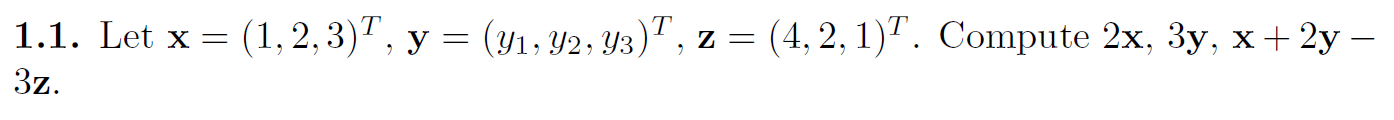
\includegraphics[width=0.9\textwidth]{1-1.png}
\end{figure}
\textbf{Solution}
\begin{align}
	&2x = \left[ 2,4,6 \right] ^T=\left[ \begin{array}{c}2\\4\\6\\\end{array} \right]  \\	
	&3y=\left[ 3y_1,3y_2,3y_3 \right] ^T=\left[ \begin{array}{c}		3y_1\\		3y_2\\		3y_3\\	\end{array} \right] \\
	&x+2y-3z = 
	\left[ 1+2y_1-12,2+2y_2-6,3+2y_3-3 \right] =\left[ \begin{array}{c}
		2y_1-11\\
		2y_2-4\\
		2y_3\\
	\end{array} \right] 
\end{align}

 \subsubsection{}
\begin{figure}[H]
	\centering
	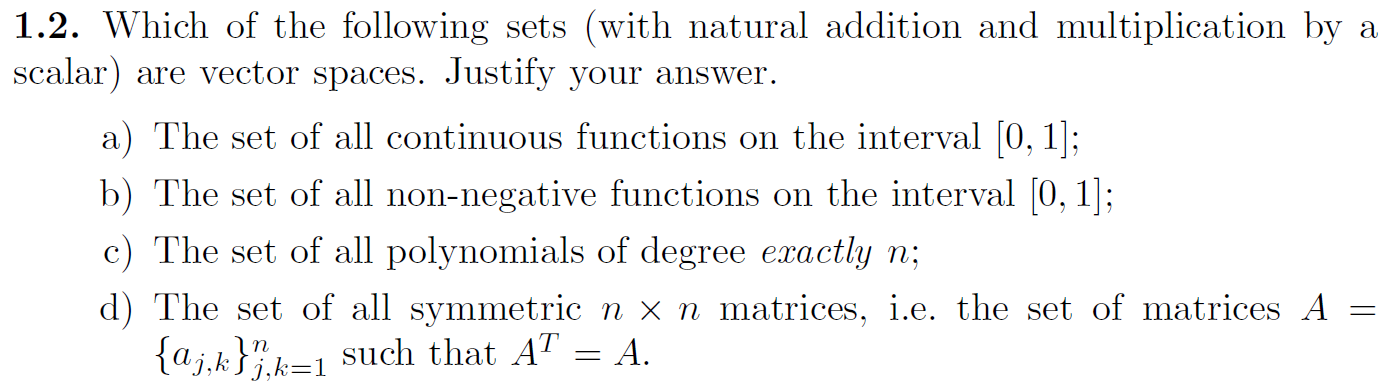
\includegraphics[width=0.9\textwidth]{1-2.png}
\end{figure}
\textbf{Solution}

 \subsubsection{}
\begin{figure}[H]
	\centering
	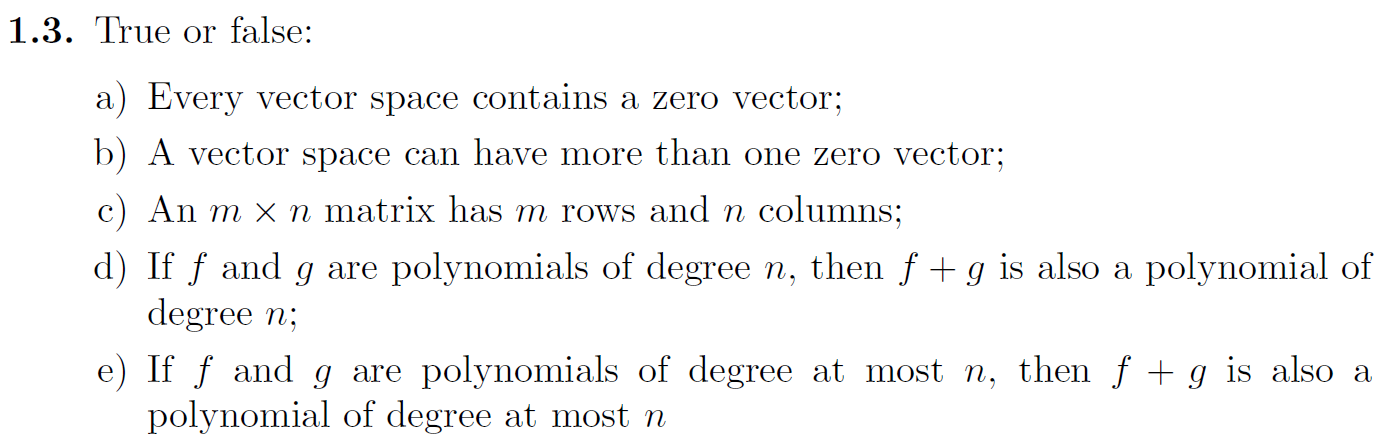
\includegraphics[width=0.9\textwidth]{1-3.png}
\end{figure}
\textbf{Solution}

	  True;	  True;	  True;	  True;	  False

 \subsubsection{}
\begin{figure}[H]
	\centering
	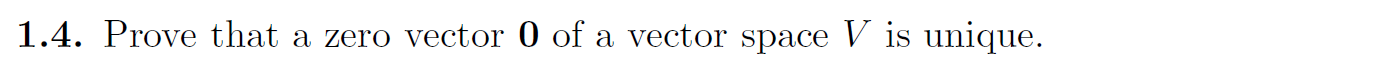
\includegraphics[width=0.9\textwidth]{1-4.png}
\end{figure}
\textbf{Solution}

\begin{assumption}
	Exist 2 different zero vectors $0_1, 0_2$. 
\end{assumption}
For any $v\in V $, we have
\begin{align}
	v + 0_1 = v\\
	v + 0_2 = v
\end{align}

So, we got 
\begin{align}
	0_1 - 0_2 = 0, \text{then } 0_1 = 0_2,\text{The zero vector is unique.}
\end{align}
 \subsubsection{}
\begin{figure}[H]
	\centering
	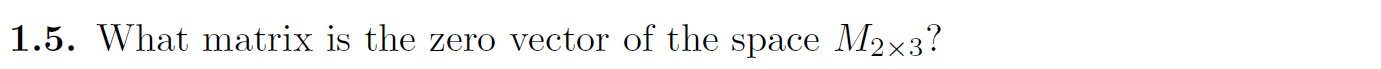
\includegraphics[width=0.9\textwidth]{1-5.png}
\end{figure}
\textbf{Solution}
\begin{align}
	O=\left[ \begin{matrix}
		0&		0    &0\\
		0&		0    &0\\
	\end{matrix} \right] 	
\end{align}
 \subsubsection{}
\begin{figure}[H]
	\centering
	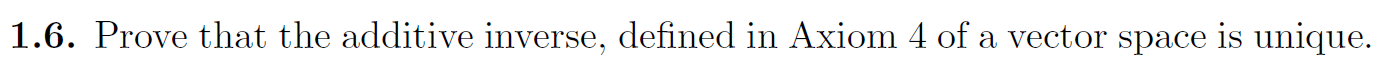
\includegraphics[width=0.9\textwidth]{1-6.png}
\end{figure}
\textbf{Solution}
\begin{assumption}
	Exist 2 different additive inverses $w_1, w_2$. 
\end{assumption}
For any $v\in V $, we have
\begin{align}
	v + w_1 = 0\\
	v + w_2 = 0
\end{align}

So, we got 
\begin{align}
	w_1 - w_2 = 0, \text{then } w_1 = w_2,\text{The additive inverse is unique.}
\end{align}
 \subsubsection{}
\begin{figure}[H]
	\centering
	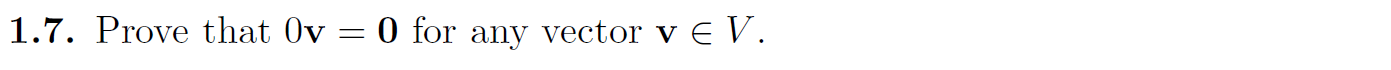
\includegraphics[width=0.9\textwidth]{1-7.png}
\end{figure}
\textbf{Solution}
\begin{enumerate}
	\item We have $v \in V$
	\item Acoording to \textbf{Multiplicative associativity}, we have $0v = (\beta 0)v = 0(\beta v)$
	\item $0v - \beta (0v) = (1-\beta)0v = 0$, so $ 0v = 0$.
\end{enumerate}
 \subsubsection{}
\begin{figure}[H]
	\centering
	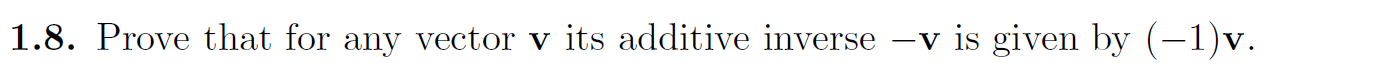
\includegraphics[width=0.9\textwidth]{1-8.png}
\end{figure}
\textbf{Solution}
\begin{enumerate}
	\item According to \textbf{1.6}: additive inverse is unique.
	\item $v - (-1)v = (1-1)v = 0$, so $(-1)v = -v$.
\end{enumerate}
\pagebreak
\subsection{Linear combinations,base.}
	\subsubsection{}
	\begin{figure}[H]
		\centering
		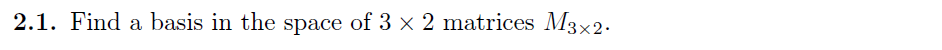
\includegraphics[width=0.9\textwidth]{1-2-1.png}
	\end{figure}
	\textbf{Solution}
	\begin{align}
		\left[ \begin{matrix}
			1&		0    \\
			0&		0    \\
			0&		0    \\
		\end{matrix} \right] 
		,
		\left[ \begin{matrix}
			0&		1    \\
			0&		0    \\
			0&		0    \\
		\end{matrix} \right] 
		,\cdots ,
		\left[ \begin{matrix}
			0&		0    \\
			0&		0    \\
			0&		1    \\
		\end{matrix} \right] 
	\end{align}
	\subsubsection{}
	\begin{figure}[H]
		\centering
		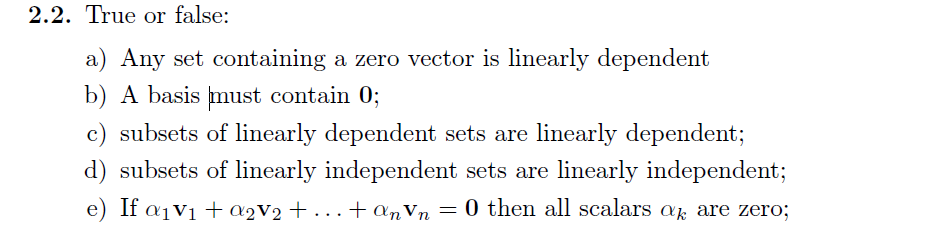
\includegraphics[width=0.9\textwidth]{1-2-2.png}
	\end{figure}
	\textbf{Solution}

	UNKNOWN; UNKNOWN; FALSE; TRUE; TRUE.
	\subsubsection{}
	\begin{figure}[H]
		\centering
		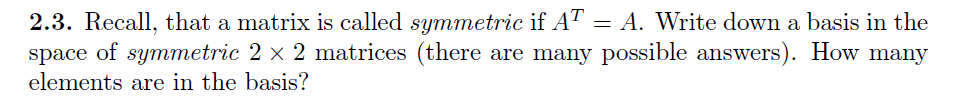
\includegraphics[width=0.9\textwidth]{1-2-3.png}
	\end{figure}
	\textbf{Solution}
	\begin{align}
		\left[\begin{matrix}
			1& 0\\
			0& 0\\
		\end{matrix}\right]
		,
		\left[\begin{matrix}
			0& 0\\
			0& 1\\
		\end{matrix}\right]
		,
		\left[\begin{matrix}
			0& 1\\
			1& 0\\
		\end{matrix}\right]
	\end{align}
	\subsubsection{}
	\begin{figure}[H]
		\centering
		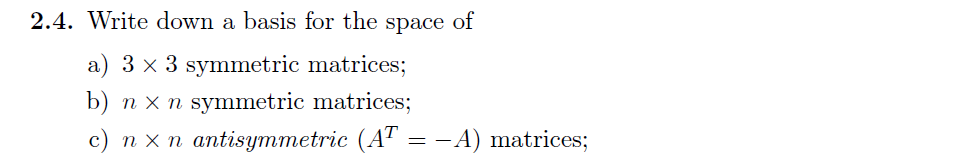
\includegraphics[width=0.9\textwidth]{1-2-4.png}
	\end{figure}
	\textbf{Solution}
	\begin{enumerate}[a)]
		\item	
		\begin{align}
			\left[\begin{matrix}
				1& 0&0\\
				0& 0&0\\
				0& 0&0\\
			\end{matrix}\right]
			,
			\left[\begin{matrix}
				0& 0&0\\
				0& 1&0\\
				0& 0&0\\
			\end{matrix}\right]
			,
			\left[\begin{matrix}
				0& 1&0\\
				1& 0&0\\
				0& 0&0\\
			\end{matrix}\right]
			,
			\left[\begin{matrix}
				0& 0&1\\
				0& 0&0\\
				1& 0&0\\
			\end{matrix}\right]
			,			
			\left[\begin{matrix}
				0& 0&0\\
				0& 0&1\\
				0& 1&0\\
			\end{matrix}\right]
			,
			\left[\begin{matrix}
				0& 0&0\\
				0& 0&0\\
				0& 0&1\\
		\end{matrix}\right]
		\end{align}
		\item And so on.
		\item 
		\begin{align}
			\left[\begin{matrix}
				1& 0&0\\
				0& 0&0\\
				0& 0&0\\
			\end{matrix}\right]
			,
			\left[\begin{matrix}
				0& 0&0\\
				0& 1&0\\
				0& 0&0\\
			\end{matrix}\right]
			,
			\left[\begin{matrix}
				0& 1&0\\
				-1& 0&0\\
				0& 0&0\\
			\end{matrix}\right]
			,
			\left[\begin{matrix}
				0& 0&1\\
				0& 0&0\\
				-1& 0&0\\
			\end{matrix}\right]
			,			
			\left[\begin{matrix}
				0& 0&0\\
				0& 0&1\\
				0& -1&0\\
			\end{matrix}\right]
			,
			\left[\begin{matrix}
				0& 0&0\\
				0& 0&0\\
				0& 0&1\\
		\end{matrix}\right]
		\end{align}
	\end{enumerate}

	\subsubsection{}
	\begin{figure}[H]
		\centering
		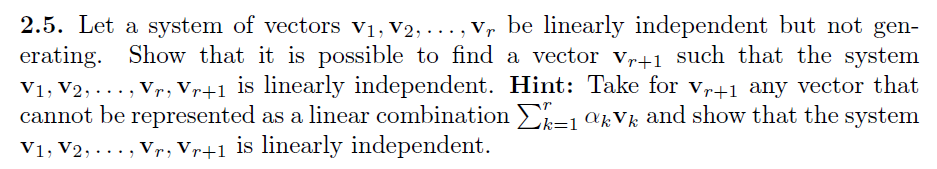
\includegraphics[width=0.9\textwidth]{1-2-5.png}
	\end{figure}
	\textbf{Solution}
	\begin{figure}[H]
		\centering
		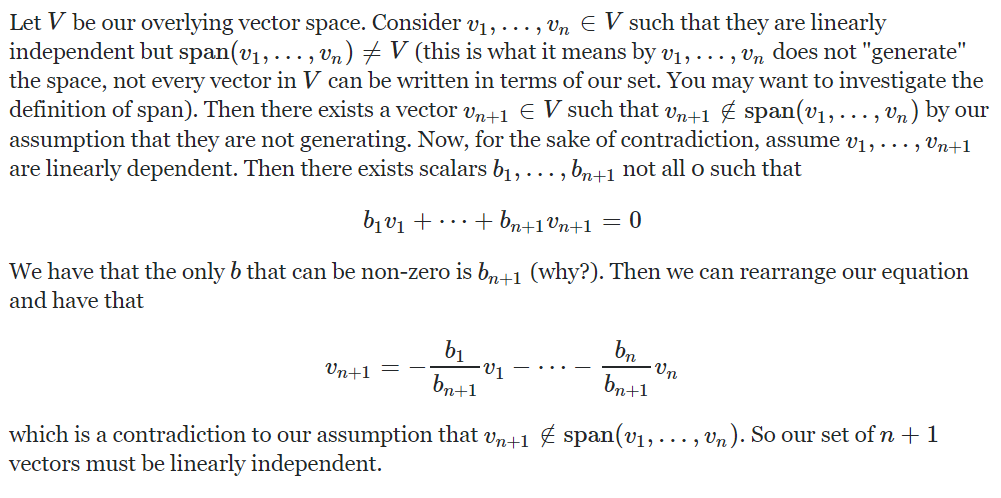
\includegraphics[width=1\textwidth]{1-2-5-1.png}
	\end{figure}

	\subsubsection{}
	\begin{figure}[H]
		\centering
		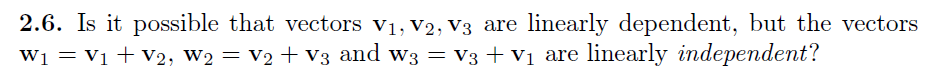
\includegraphics[width=0.9\textwidth]{1-2-6.png}
	\end{figure}
	\textbf{Solution}
	\begin{enumerate}
		\item According to the statement, we can get
		\begin{align}
			\begin{cases}
				\alpha _1v_1+\alpha _2v_2+\alpha _3v_3=0\\
				\beta _1\left( v_1+v_2 \right) +\beta _2\left( v_2+v_3 \right) +\beta _3\left( v_1+v_3 \right) =0\\
			\end{cases}\rightarrow \begin{cases}
				\alpha _1=\beta _1+\beta _3 = 0\\
				\alpha _2=\beta _2+\beta _3 = 0\\
				\alpha _3=\beta _1+\beta _2 = 0\\
			\end{cases}
		\end{align}
		\item We can know that $\beta_1,\beta_2,\beta_3$ can be arbitrary. So, it is impossible to be linearly independent.
	\end{enumerate}
\end{document}
%===结束===



